\documentclass[12pt]{article}
\usepackage{charter} % font
\usepackage[margin=1in]{geometry} % margin
\usepackage{hyperref} % hyperlinks
\usepackage{enumitem} % Enumeration
\usepackage{graphicx} % images
\graphicspath{ {.} } 

\usepackage[lined,dotocloa]{algorithm2e} % Pseudocode
\labelformat{algocf}{\textit{alg.}\,(#1)}


%%%%%%%%%%%%%%%%%%%%%%%%%%%%%%%%%%%%%%%%%%%%%%%%%%%%%%%%%%%%%%%%%%%%%%%%%%%%%%%%

\title{%
	\textbf{Assignment 3 \\ 
	Sorting: Putting your affairs in order \\
	\large WRITEUP} }

	\author{Zack Traczyk \\ CSE13S - Spring 2021}
	\date{Due: April 25\textsuperscript{th} at 11:59 pm}

%%%%%%%%%%%%%%%%%%%%%%%%%%%%%%%%%%%%%%%%%%%%%%%%%%%%%%%%%%%%%%%%%%%%%%%%%%%%%%%%

	\begin{document}

	\maketitle

	\section{Time Complexity}

	\subsection{Bubble Sort}

	For larger arrays, Bubble Sort had the worst time complexity out of all the sorts implemented.
	Figure \ref{bubble} displays the relationship between the amount of comparisons the algorithm performs for the number of items of the given array.
	As shown, Bubble Sort has a worst case complexity of $O(n^2)$ as it has two nested for loops that usually iterate through the entirety of the array.
	
	A reversed array requires the most amount of comparisons in bubble sort.

	The corresponding $C$ value for bubble sort is 

		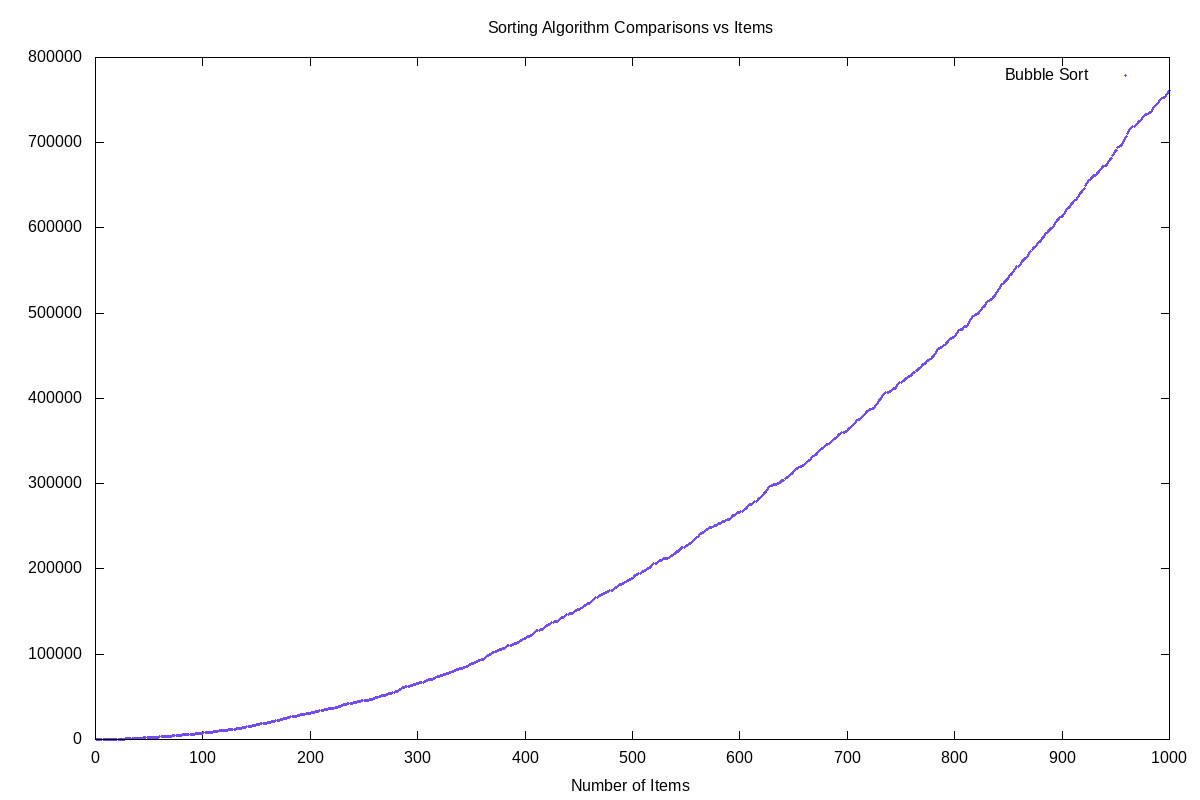
\includegraphics[width=\textwidth]{bubble} \label{bubble}

	\subsection{Shell Sort}

	Shell sort preformed much better than Bubble Sort. Figure \ref{bubble}.

	Reverse

		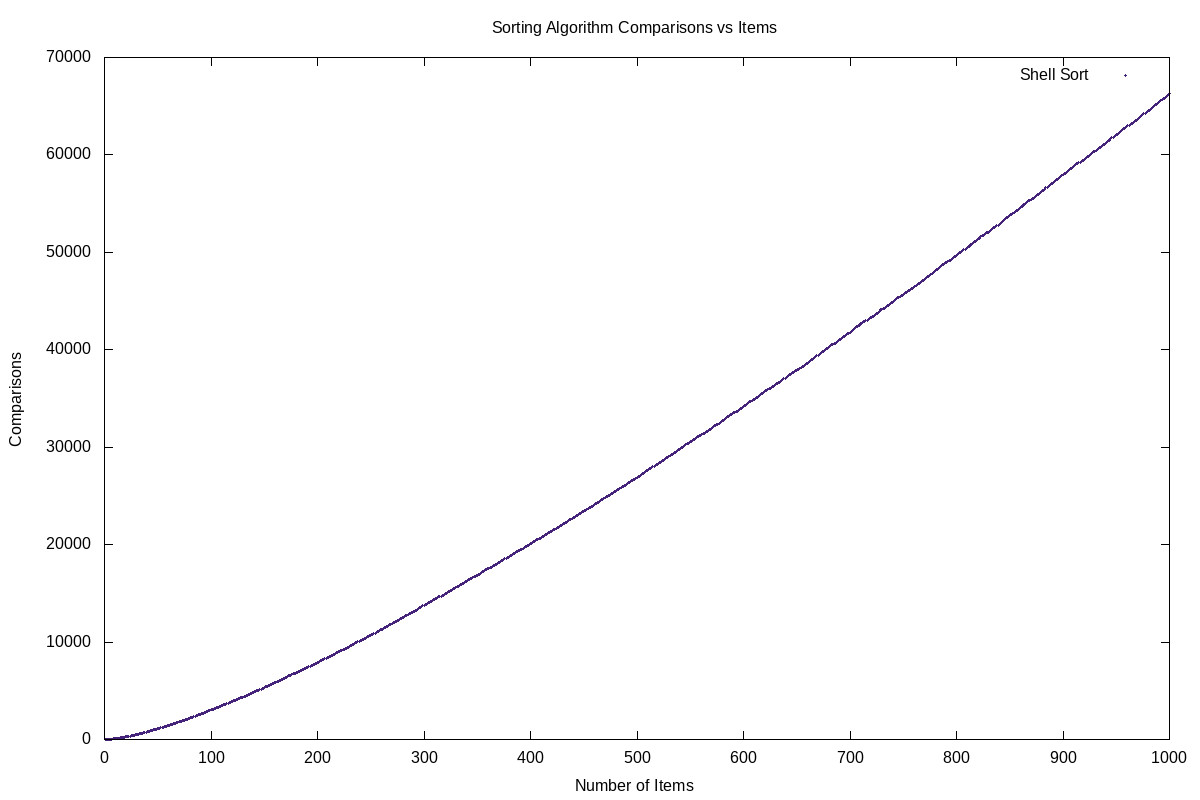
\includegraphics[width=\textwidth]{shell} \label{shell}

	\subsection{Quick Sort}

	Shell sort preformed much better than Bubble Sort. Figure \ref{stack}. Figure \ref{queue}

		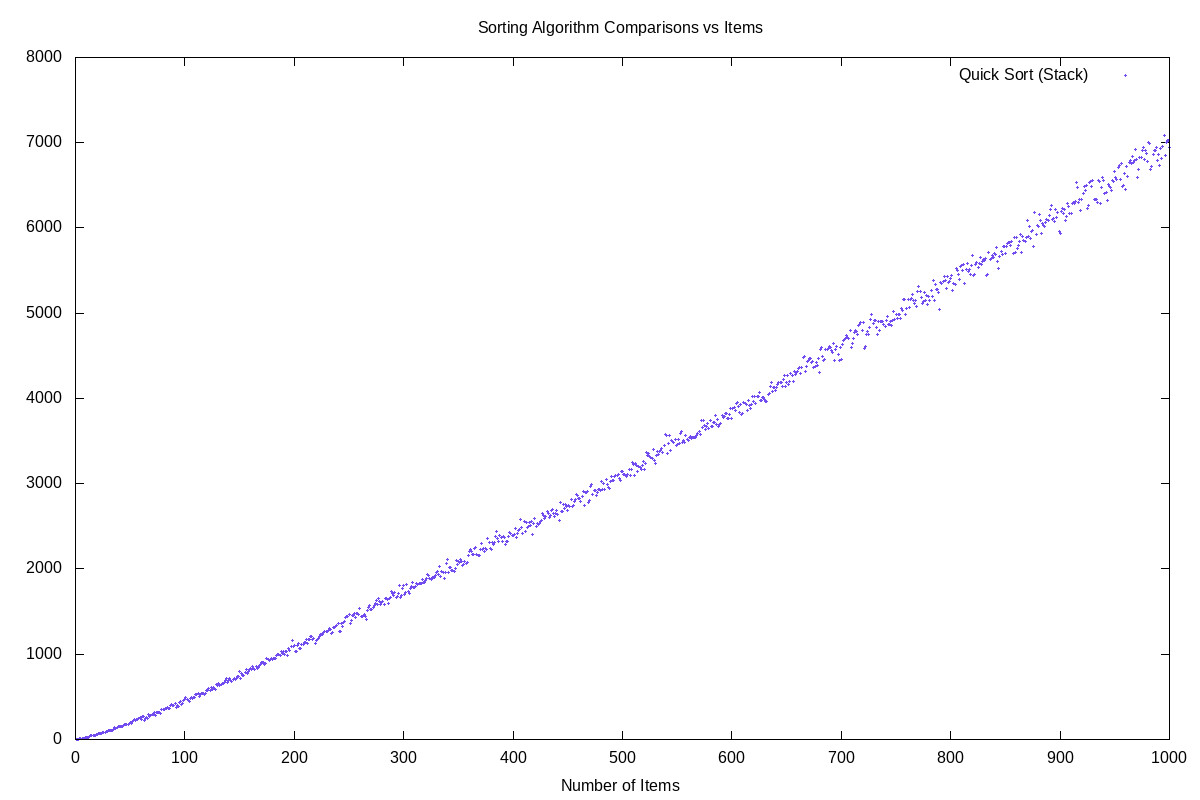
\includegraphics[width=\textwidth]{quick_stack} \label{stack}

		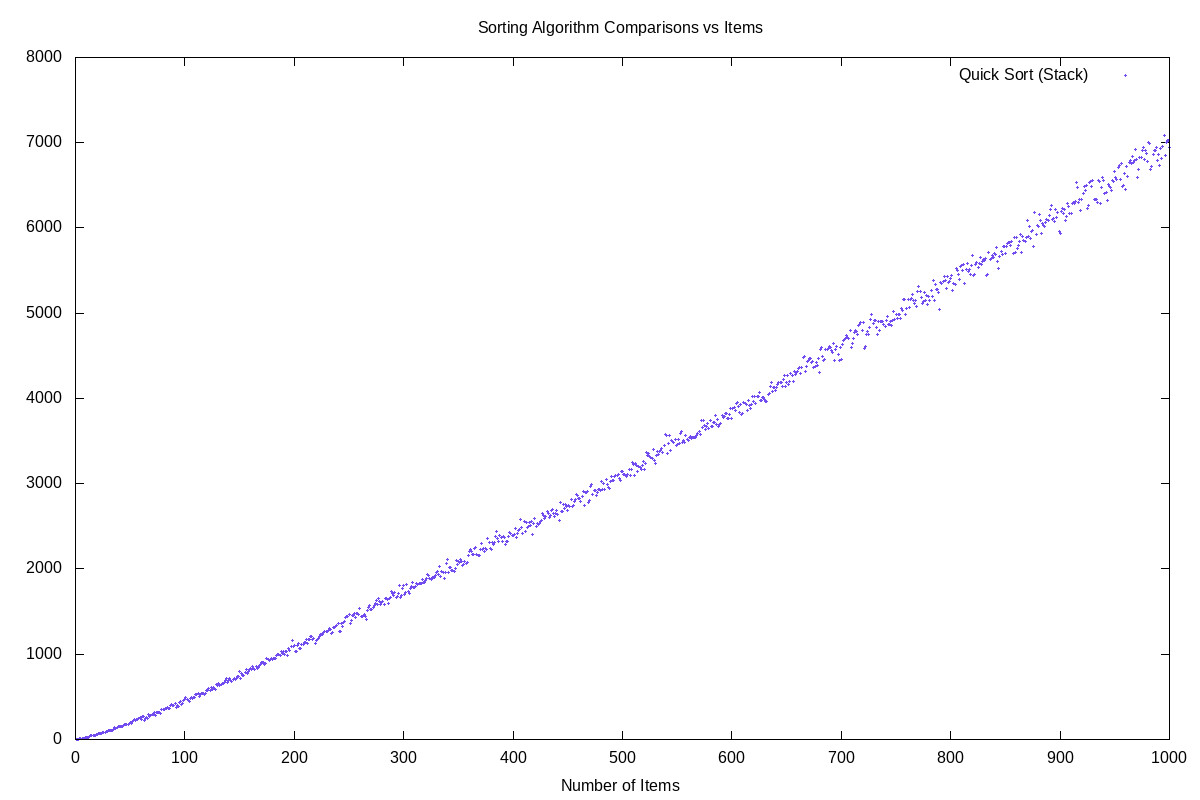
\includegraphics[width=\textwidth]{quick_stack} \label{queue}

	More graphs

	\section{What I Learned}

	Picking the right algorithm is crucial for accomplishing fast code. Furthermore, right does not necessarily mean smallest Big-$O$ or even the fastest. It is about considering memory usage, and size of array.

	\end{document}

